\begin{frame}[fragile]
  \frametitle{Planteamiento del Problema}
  
  \begin{alertblock}{El problema en la región Caribe}
    18 estaciones meteorológicas distribuidas en 404,7 km × 252,2 km\\
    \textbf{Densidad:} 1,8 estaciones por 10.000 km² $\Rightarrow$ insuficiente
  \end{alertblock}
  
  \begin{itemize}
    \small
    \item Datos dispersos no describen el estado continuo
    \item Vacíos de información en zonas sin instrumentación
    \item Necesidad de estimar presión y viento
  \end{itemize}
  
  \note[item]{Pregunta: ¿Cómo reconstruir campos atmosféricos desde datos dispersos?}
  \note[item]{Tiempo: 2-3 minutos}
\end{frame}

\begin{frame}[fragile]
  \frametitle{Planteamiento del Problema: Distribución de Estaciones}

  \begin{center}
    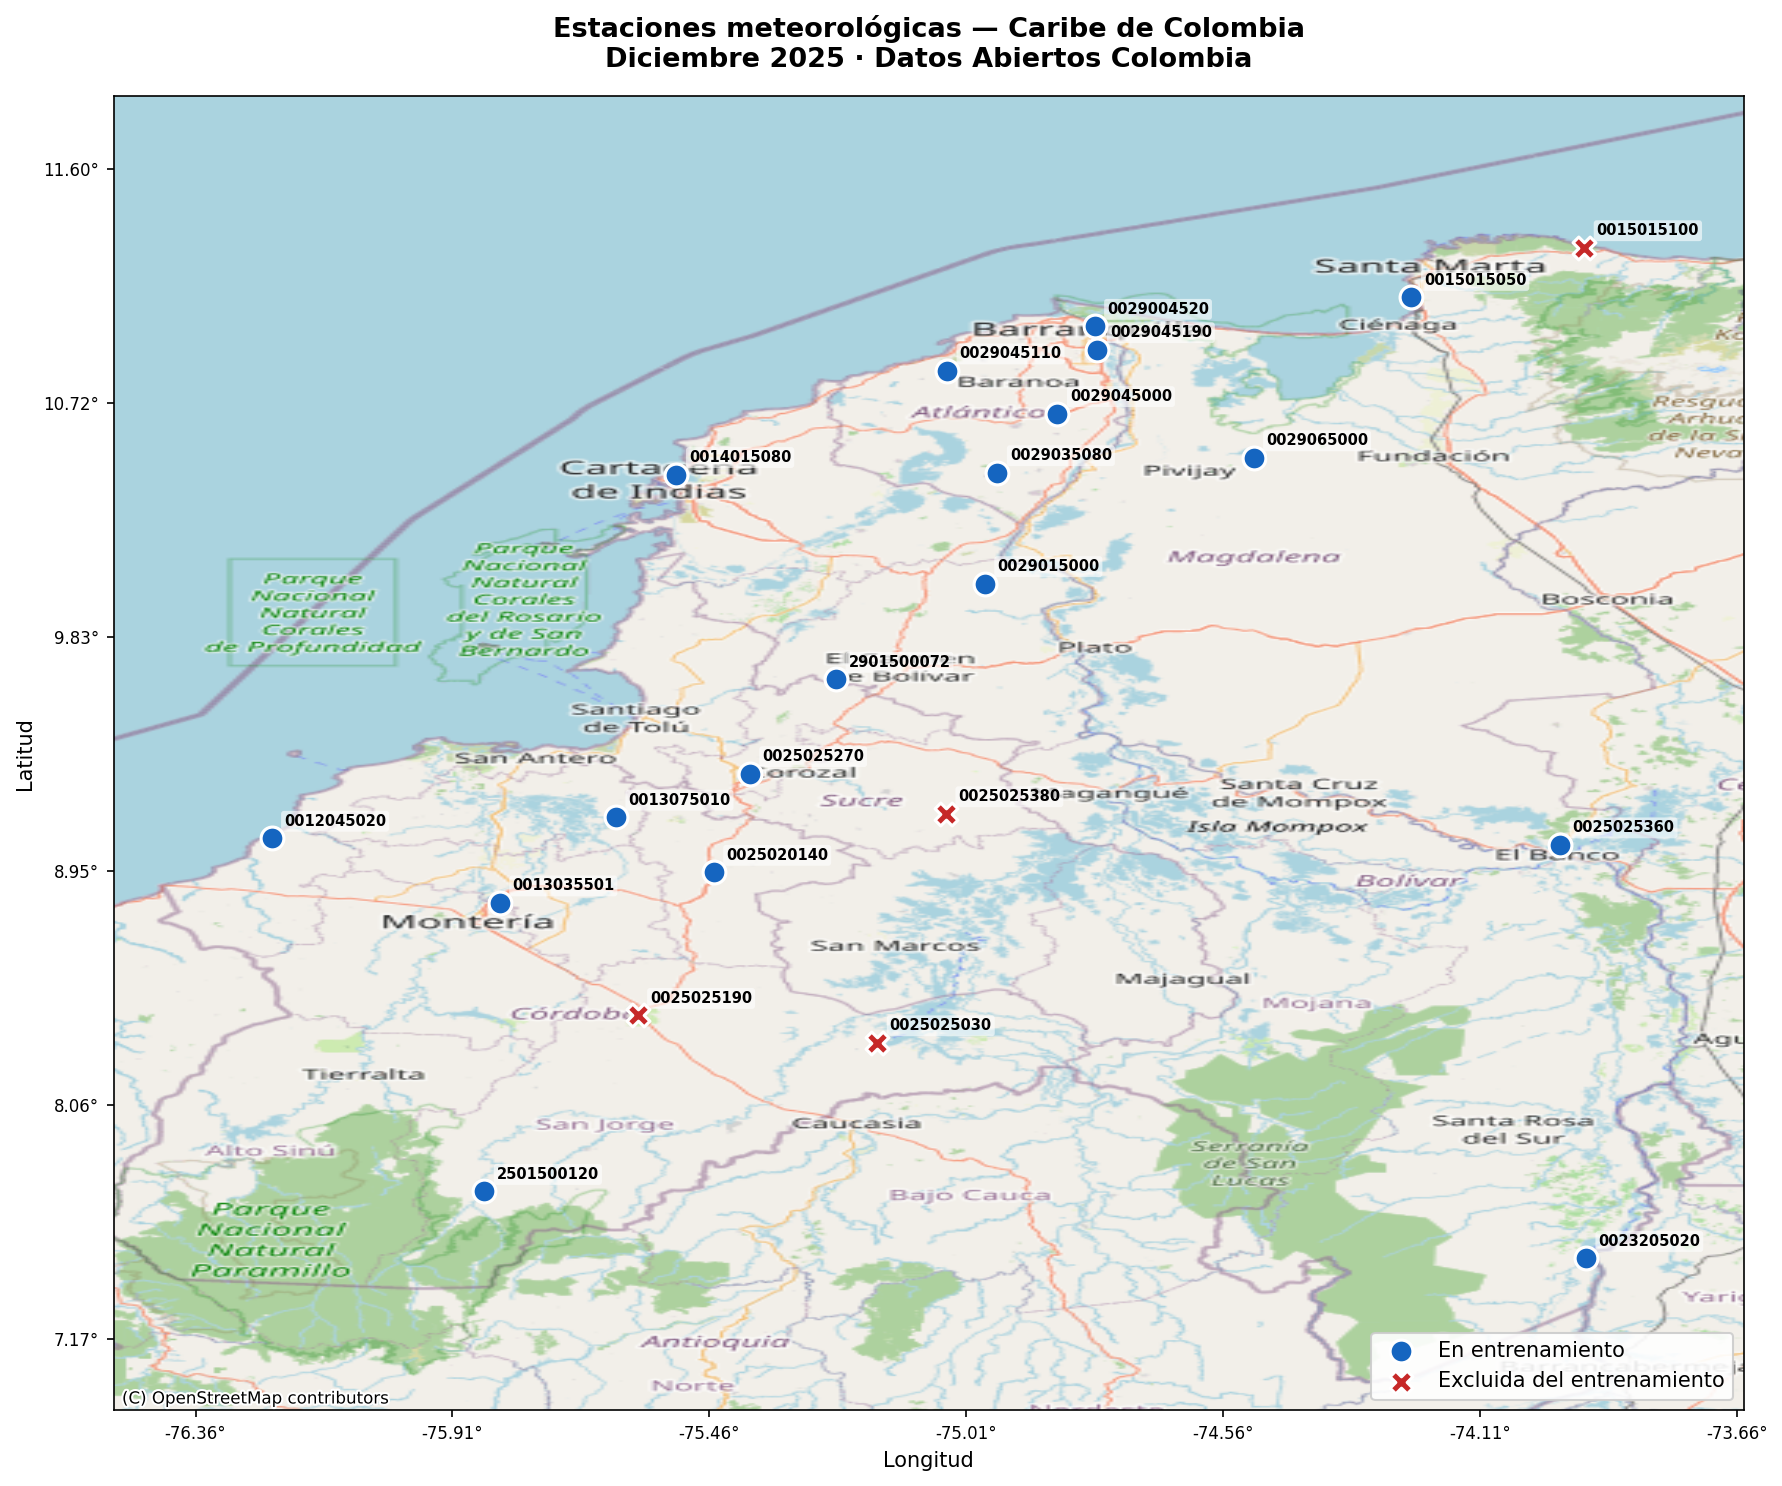
\includegraphics[width=0.85\textwidth]{figures/mapa_estaciones_caribe.png}
  \end{center}

  \note[item]{Mapa de cobertura espacial de las 18 estaciones meteorológicas en la región Caribe.}
\end{frame}

\begin{frame}[fragile]
  \frametitle{Pregunta de Investigación}

  \begin{block}{Pregunta central}
    \centering
    \large
    ¿Cómo construir un modelo basado en PINNs que, a partir de registros meteorológicos dispersos y de las ecuaciones de Navier-Stokes, permita estimar la presión y las componentes del viento sobre una malla espacio-temporal en puntos donde no existen estaciones de medición?
  \end{block}

  \note[item]{Conectar el problema de cobertura espacial con la necesidad de un modelo físicamente consistente.}
\end{frame}
